\documentclass{sls-note}
\usepackage{graphicx}
% \usepackage{a4wide}
\title{Simulations for Touschek Lifetime}
\author{Helge Kr\"uger}

\begin{document}
%%%%%%%%%%%%%%%%%%%%%%%%%%%% SLS Title Page %%%%%%%%%%%%%%%%%%%%%%%%%%%%%%%%%
\slstitle{
  SLS-TME-TA-2005-0283
}{
  Simulations for Touschek Lifetime
}{
  Helge Kr\"uger
}{
  \PSI \\(Summer student from University of Vienna)
}{
  \slsabstract{Single intrabeam scattering of electrons leading to energy changes larger than the energy acceptance (Touschek scattering) is an important mechanism of particle loss in a light source storage ring. The dependance of Touschek lifetime on beam properties (emittance, coupling, bunch length etc.) and energy acceptance can be described by an analytical formula, which has proven to agree well with observations at existing machines. This formula describes an obvious decrease of Touschek lifetime with shrinking emittance, however for ultralow emittance beams, the lifetime should become larger again.\\ This report deals with the modeling of Touschek effect based on macro particles. Different approaches like direct Coulomb scattering and M{\o}ller scattering will be discussed. Results for a simple test lattice and the SLS lattice will be compared to the analytical formula and to measurements done at SLS. 
}}
%  During my stay as a summer student, I wrote a simulation to compute the Touschek Lifetime. This document gives an overview over what I did. We also conducted measurements with the SLS to validate my computations.
%%%%%%%%%%%%%%%%%%%%%%%%%%%%%%%%%%%%%%%%%%%%%%%%%%%%%%%%%%%%%%%%%%%%%%%%%%%%%

% \maketitle
\tableofcontents
\section{Introduction}
The aim of this document is to give an overview over what I have done during my time as a summer student at the Paul Scherrer Institut in Villigen. I was there during the summer 2005. My task was to write a simulation for the Touschek Effect in a storage ring, with the goal to do simulations for the ultra low emmitance case.
\subsection{What is the Touschek Effect?}
The effect of electreons being lost from a stored beam due to intra beam scattering is called Touschek Effect. Here transversal momenta is transfered into longitudinal momenta. This effect is amplified by a $\gamma$-factor, causing the electrons to fall out of the momenta acceptance of the storage ring.
\subsection{Description}
Up to now people have used different 2 main different approaches to describe the Touschek Effect. People have derived analytical formulas using different assumptions. For a choice of 2, you can look at section ``Analytical Touschek Effect''. And S. Khan did something similar to our calculations.

\section{Theory}
\subsection{Linear Beam Optics}
In order to simulate the storage ring, we are using linear beam optics as described in [5]. However we are using a 6 dimensional model there and not a 4 dimensional model as described there. Our transformation matrix for a combined function magnet is given by:
\begin{equation} M = \left( \begin{array}{cccccc}
\cos \phi_x & \frac \rho {\sqrt{1 - n}} \sin \phi_x & 0 & 0 & 0 & \frac \rho {1 - n} (1 - \cos \phi_x) \\
- \frac{\sqrt{1 - n}} \rho \sin \phi_x & \cos \phi_x & 0 & 0 & 0 & \frac 1 {\sqrt{1 - n}} \sin \phi_x \\
0 & 0 & \cos \phi_y & \frac \rho n \sin \phi_y & 0 & 0 \\
0 & 0 & - \frac {\sqrt n} \rho \sin \phi_x & \cos \phi_x & 0 & 0 \\
- \frac 1 {\sqrt{1 - n}} \sin \phi_x & - \frac \rho {1- n } (1 - \cos \phi_x) & 0 & 0 & 1 & \frac \rho {(1 - n)^{3/2}} - \frac L {1 - n} \\
0 & 0 & 0 & 0 & 0 & 1 \end{array} \right) \end{equation}
with $\phi_x = \rho \sqrt{1 - n}$, $\phi_y = \phi \sqrt n$ and $L = \phi \cdot \rho$, where $\rho$ is the radius of the magnet, $\phi$ is the angle and n the field index.\\
Our cavity matrix is given by:
\begin{equation} M = \left( \begin{array}{cccccc}
1 & 0 & 0 & 0 & 0 & 0 \\
0 & 1 & 0 & 0 & 0 & 0 \\
0 & 0 & 1 & 0 & 0 & 0 \\
0 & 0 & 0 & 1 & 0 & 0 \\
0 & 0 & 0 & 0 & 1 & 0 \\
0 & 0 & 0 & 0 & \frac {\Delta E} E & 1 
\end{array} \right). \end{equation}
Where we have:
\begin{equation} \frac{\Delta E} E = \frac{2 \pi e V \cos \phi_s}{E \lambda} \end{equation}
where $\phi_s$ is the phase.
\subsection{Beam Matching}
To do the matching we proceed as follows. We have the linear map:
\begin{equation}
\left( \begin{array}{c}z \\ z' \end{array} \right)_f =
\left( \begin{array}{cc} A & B \\ C & D \end{array} \right) \cdot
\left( \begin{array}{c}z \\ z' \end{array} \right)_i .
\end{equation}
We then put:
\begin{equation}
\left( \begin{array}{cc} A & B \\ C & D \end{array} \right) =
\left( \begin{array}{cc} \cos \mu_s & - \beta_s \sin \mu_s \\ 
\frac 1 {\beta_s} \sin \mu_s & \cos \mu_s \end{array} \right).
\end{equation}
And we get the standard deviations of the beam with:
\begin{eqnarray} \sigma_z &=& \sqrt{\epsilon_z \beta_z} \textnormal{ and}\\
\sigma_{z'} &=& \sqrt{\frac{\epsilon_z}{\beta_z}}.
\end{eqnarray}
Something similar should work for the x and y direction. The transformation matrix is the one for the whole storage ring, the one turn map. See [5] for more information.

\subsection{Debye Length}
In approximations we often need a characteristic length. For this we can use the Debye Length, given by:
\begin{equation} \lambda_D = \left(\frac{\epsilon_0 k_B T}{q^2 n} \right)^2 \end{equation}
where T is the temperature, q the charge and n the density. In the theory of plasmas (and also for nonneutral plasmas) the Coulomb potential is shielded, if 2 electrons are farther apart then $\lambda_D$.\\
For more Information on the Debye Length see [1] Section 3.4 page 59 or [2] begins of chapter 4 page 186.\\
When we were doing particle - particle interactions we restricted our self to interactions where the distance was smaller, then the Debye length.

\subsubsection{Temperature of a relativistic beam}
In our formula for the Debye Length $\lambda_D$, it is not clear what the temperature is. Actually for our beam we have several temperatures, like the transversal and longitudinal temperatures. We also need to pay attention to in which frame we compute the temperature. However the beam is much smaller in the transversal direction, then in the longitudinal directions. Especially since by transforming to the beam frame, the beam becomes bigger by a factor of $\gamma$ in the longitudinal direction. So we can take the transversal temperature, which is given by:
\begin{equation} k_B T = m \overline{v_\perp ^2} \end{equation}
in the beam frame. To transform into the laboratory frame, the m goes to $\gamma m$.

\subsection{Relativistic considerations and effects}
In our simulation we use 3 frames of reference. One is the laboratory frame, one is the beam or bunch frame and one is the center of momentum frame. The laboratory frame is moving with the beam, so turning around with it, and moving. The beam frame is the one where the reference particle is at rest. So the difference between these 2 is a Lorentz transformation with the beam velocity in transversal direction to the beam.\\
The center of momentum frame is always different for the particles. In it the center of mass of the 2 particles is at rest, so they are only in relative motion, with speeds opposite to each other. This is for example necessary to compute the cross section.

\subsubsection{Lorentz Transformation}
To pass from the laboratory frame to beam frame, we have to use the Lorentz transformation, so we have:
\begin{eqnarray}
\beta &=& \frac v c \\
\gamma &=& \left(1 - \beta^2\right)^{-1/2}
\end{eqnarray}
\begin{equation}
\left(\begin{array}{c}t\\x\\y\\s \end{array}\right)_B =
\left( \begin{array}{cccc}
\gamma & 0 & 0 & - \beta \gamma \\ 
0 & 1 & 0 & 0 \\ 
0 & 0 & 1 & 0 \\ 
- \beta \gamma & 0 & 0 & \gamma 
\end{array} \right) 
\cdot \left(\begin{array}{c}t\\x\\y\\s\end{array} \right)_L.
\end{equation}
This mainly leads to the bunch become larger by a factor of $\gamma$ in the beam frame. Also note, that the relativistic momentum is given by:
\begin{equation}
p = (\gamma m_0 c, \gamma m_0 v^1, \gamma m_0 v^2, \gamma m_0 v^3)
\end{equation}
and that it transforms like the coordinate, so:
\begin{equation} p_B = \Lambda \cdot p_L \end{equation}
with $\Lambda$ the 4 x 4 Matrix above.
\subsection{Momentum Coordinate and collision}
For the coordinates for the momentum we use relative unit less coordinates, so from the real momentum $p_z$ to our coordinate $z'$ we transform with:
\begin{equation} z' = \frac{p_z - p_{0}}{p_{0}} = \frac{p_z}{p_0} - 1 \end{equation}
where $p_{0}$ is a reference momentum in the z direction. Taken here as $p_{0} = \gamma m_0 \beta c$. For the transversal coordinates we have:
\begin{equation} x' = \frac{p_x}{p_0} \ , \ y' = \frac{p_y}{p_0} \ , \ p_0  = \gamma m_0 \beta c. \end{equation}
To do the collision only the longitudinal coordinate gets transformed by a Lorentz transformation so we have, with E the energy:
\begin{equation} (E, p) \rightarrow (E', p') = (\gamma E - \beta \gamma p, \gamma p - \beta \gamma E). \end{equation}
Then the collision leads to a momentum change by $\Delta p$, so we have:
\begin{equation} p' \rightarrow p' + \Delta p. \end{equation}
This gets back transformed into the laboratory system leading to:
\begin{equation} p_{new} = p + \gamma \Delta p = p_0 + z' \cdot p_0 + \gamma \Delta p.\end{equation}
So this would lead us to a change in the coordinate z' by
\begin{equation} z' \rightarrow z' + \frac{\gamma \Delta p}{p_0}. \end{equation}
Using that $\Delta p = m_0 \cdot \Delta v$ and $p_0 = \gamma m_0 \beta c$ we get:
\begin{equation} z' \rightarrow z' + \frac{\Delta v}{\beta c}. \end{equation}

\subsubsection{Why we need to be fully relativistic}
The relativistic speed is given by:
\begin{equation}u^i = \frac{dx^i}{d\tau}. \end{equation}
Where $\tau$ denotes the proper time. The momentum is then $p = m u$, so we get in the laboratory system: $p = \gamma m v$ where v is the velocity measured in the laboratory system. The x and y components of the velocity aren't transformed when passing to the beam system, so we still have the same there. Assuming we would be able to calculate using classical mechanics, we would have $p = m v$ so $v_B = m v_L$ with $v_L \approx 10^5 m / s$ we would run to speeds bigger then the speed of light, for $\gamma > 3000$, which is a more then realistic value where we want to do the calculations.

\subsection{Quantum Electrodynamics}
The cross section we are using for electron electron scattering comes from quantum electrodynamics, it is given by:
\begin{equation} \sigma = \frac{d\sigma}{d\Omega} = \frac{r_e ^2}{4} \left(1 - \frac{v^2}{c^2}\right) \left[ (X+1)^2 \left(\frac 4 {\sin^4 \Theta} - \frac 3 {\sin^2 \Theta}\right) + 1 + \frac 4 {\sin^2 \Theta}\right] \end{equation}
with
\begin{equation} X = \left(\frac c v\right)^2 = \beta^{-2} = \frac{\gamma^2}{\gamma^2 - 1}. \end{equation}
It is derived assuming that the scattering process is done by the exchange of one photon. This formula is called M{\o}ller-Scattering, because M{\o}ller was the first to derive it. For a derivation of this cross section consult [13].

\begin{figure}[here]
 \centering
 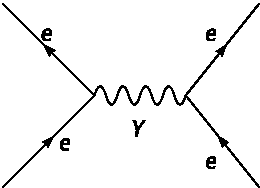
\includegraphics[width=0.50\textwidth]{inter.pdf}
 \caption{Feynman Diagram of the interaction}
\end{figure}


This cross section formula is valid in the center of momentum frame of both electrons.

\subsection{Analytical Touschek Effect}
There are some analytical results on the Touschek effect, so we have formulas for how many particles are left after a certain time. To compute this, one assumes the following:
\begin{equation}\frac{dN}{dt} = - \alpha N^2. \end{equation}
This is reasonable, because each particle has N possible particles to scatter of, so we got a total of $N^2$ of chances of a particle being lost. This leads to the function of particles in time, given by:
\begin{equation} N(t) = N_0 \cdot \frac 1 {1 + N_0 \alpha t} \end{equation}
with $N_0$ the number of particles at the time 0. The half lifetime is given by:
\begin{equation}\tau_{1/2} = - \frac{N(0)}{\dot N(0)} = \frac 1 {\alpha N(0)}. \end{equation}
\subsubsection{Classical Formula}
After Andreas Streun in [3], the factor $\alpha$ is given by:
\begin{equation} \alpha = \frac{r_0 ^2 c}{8 \pi \gamma^3 \sigma_s} \frac{F\left(\left(\frac{\delta_{acc}}{\gamma \sigma_{x'}}\right)^2\right)}{\sigma_x \sigma_y \sigma_{x'} \delta_{acc} ^2}. \end{equation}
  \begin{itemize}
  \item $r_0$ the classical electron radius.
  \item $\delta_{acc}$ the momentum acceptance.
  \item $\sigma_x$ the standard deviation of the bunch size.
  \item $\sigma_{x'} = \frac{\epsilon_x}{\sigma_x} \sqrt{1 + H \cdot \frac{\sigma_{t'} ^2}{\epsilon_x}}$ is the rms divergence of the $p / p_0$ at $x = 0.$
  \item $F(x) = \int\limits_0^1 \left(\frac 2 u - \ln \frac 1 u -2\right) e^{-x / u} du$
  \end{itemize}
\subsubsection{V\"olkel's Approach}  
Following Uta V\"olkel in [11] the parameter $\alpha$ for a gaussian distributed beam is given by:
\begin{eqnarray}
\alpha &=& \frac {4 \pi r_0 ^2 c}{V \Delta p_{max} ^2} \cdot J \\
J &=& \int\limits_\eta^{\delta p} \frac{\sqrt{1 + p_x ^2}}{p_x} \left(1 + \frac{p_x ^2}{1 + p_x ^2}\right)^2 F(p_x) d p_x - \frac 3 4 F(0) \\
F(p_x) &=& \frac{1}{2 \sqrt \pi \delta q} e^{- \left(\frac{p_x}{\delta q}\right)^2}. 
\end{eqnarray}
Here V is the volume of the bunch in the lab system. $\delta q$ is the rms of transverse momenta in units of $m_0 c$. This means that $\delta q \approx \gamma \sigma_{x'}$, and $\delta p$ is the maximal transverse momenta, given by $\delta p = \sqrt{3} \delta q$. $\Delta p_{max}$ is the momentum acceptance and $\eta = \Delta p_{max} / \gamma$.For more details see [11]. The 2 approaches at calculating the factor $\alpha$ gives about to the same result.

\subsection{Scattering at an angle}
Here we are following what S. Khan did in [10]. We want to scatter 2 electrons by the polar angle $\Theta$ and the azimuthal angle $\Phi$. Our electrons have the momenta in the laboratory frame:
\begin{equation} \vec p_{L} = \gamma m_0 \beta c (x', y', z' + 1).\end{equation}
We now first Lorentz transform this to the bunch system. Leading us to:
\begin{equation} p_{xB} = p_{xL},\ \ p_{yB} = p_{yL},\ \ p_{zB} = \gamma p_{zL} - \beta \gamma \sqrt{p_L ^2 + m_0^2 c^2}.\end{equation}
Till now  $\beta$ and $\gamma$ were used for the transformation from laboratory to the bunch system. Now, we will use them to transform from the bunch system into the center of mass system.\\
The energy of one electron is given by:
\begin{equation} E = \sqrt{ p ^2 c^2 + m_e ^2 c^4}. \end{equation}
It is different for the 2 electrons. The relativistic parameters to transform into the center of momenta system are given by:
\begin{equation} \vec \beta = \frac{\vec p_1 + \vec p_2}{E_1 + E_2} c \end{equation}
and we can obtain $\gamma$ by:
\begin{equation} \gamma = \frac 1 {\sqrt{1 - \beta^2}} \end{equation}
We have the transformation
\begin{equation} \vec q_i = \vec p_i + \vec \beta \gamma \left[ \frac \gamma {\gamma + 1} \vec \beta \vec p_i - \frac{E_i}{c}\right] \end{equation}
and the back transformation
\begin{equation} \vec \beta \rightarrow - \vec \beta  \end{equation}
and using the right energy $E = \sqrt{ p^2 c^2 + m_e ^2 c^4}$.\\

We rotate the vector $\vec q$ into the z direction, do the scattering and transform it back, so we have:
\begin{equation} \theta = \cos^{-1} \frac {q_z} q \ \ \phi = \frac \pi 2 + \tan^{-1} \frac {q_y}{q_x} \ \ \ \psi = 0. \end{equation}
We also need to consider, that in case of $q_z < 0$, $\theta \rightarrow \theta + \pi$.\\
And we get as a vector $\vec q'$ after the scattering:
\begin{equation} \vec q' = \left(\begin{array}{ccc}
\cos \phi & - \cos \theta \sin \phi & \sin \theta \sin \phi \\
\sin \phi & \cos \theta \cos \phi & - \sin \theta \sin \phi \\
0 & \sin \theta & \cos \theta \end{array} \right) \cdot q \cdot
\left( \begin{array}{c} \sin \Theta \cos \Phi \\ \sin \Theta \sin \Phi \\ \cos \Theta \end{array} \right) \end{equation}
where q denotes the length of the vector $\vec q$ before the collision.\\
We then apply the back transform (twice! first to the bunch, then to the lab) and check if we are outside the momentum acceptance.

\subsection{Idea behind the cross section}
The main idea behind the cross section is to solve the integral for the lost rate given by:
\begin{equation} \dot N = \frac 1 {\gamma C} \int\limits_0^C ds \\
\int\limits_{-\infty}^\infty dx dy dz \\
\int\limits_{-\infty}^\infty dx'_1 dy'_1 dz'_1 \\
\int\limits_{-\infty}^\infty dx'_2 dy'_2 dz'_2 \\
\int\limits_{4 \pi} d(\cos\Theta) d\Phi 2v \sigma \rho_1 \rho_2. \end{equation}
Here we are integrating over a 12 dimensional volume. $d(\cos \Theta) d\Phi = d\Theta d\Phi \sin \Theta$ is an area element in the angle coordinates. $\int_{-\infty}^\infty dx dy dz$ is the integration over all possible positions where the interaction could take place. $\int_{-\infty}^\infty dx'_1 dy'_1 dz'_1$ and $\int_{-\infty}^\infty dx'_2 dy'_2 dz'_2$ over the possible momenta of the 2 interaction partners. $\int_0^C ds$ is the integral along the storage ring, because the parameters before depend on where you are in the ring.
\subsection{Idea behind Monte Carlo Integration}
The idea behind Monte Carlo Integration is that, for n points $u_1, ..., u_n$ picked at random in the interval $\left[u, u + \Delta u\right]$, we have that:
\begin{equation} \int\limits_u^{u + \Delta u} f(u) du \approx \frac{\Delta u}{n} \sum\limits_{k=1}^n f(u_k). \end{equation}
This way we hope to solve our above integral, applying the same procedure to the multidimensional integral above. To be exact this is what Khan did in [4]. We are additionally adding in particle tracking.

\section{Direct Monte Carlo Simulation}
This approach has failed. However, it is still presented here to give people who want to try it again, about what to do and what not to do.
\subsection{Coulomb Force}
The coulomb force works between 2 charges, here 2 electrons. It is given by:
\begin{equation} \vec F = \frac {q^2} {4 \pi \epsilon_0} \cdot \frac {\vec r_1 - \vec r_2}{|\vec r_1 - \vec r_2|^3}. \end{equation}
To compute this force we have to transform to the beam frame. In the laboratory frame we would also have to do with magnetic fields. This mainly means, that the longitudinal component goes into the calculations with a factor of $\gamma$.

\subsection{Electron - Electron Scattering}
For the electron - electron scattering in a plane, I am using the formulas given by [6]. I assume that we are having strong and complete collisions. So I get for the longitudinal velocity shift after (6.10.4):
\begin{equation} \Delta v_z \approx \frac{m v^3 b_z}{2 C_0 (1 + q_c)} \end{equation}
where $C_0 = q^2 / 4 \pi \epsilon_0$ and $q_c = (m b v^2/2 C_0)^2 = (m/2C_0 \cdot b v^2)^2 \approx 10^8$ which means that the last equation can further be approximated by $1 + q_c \approx q_c$ to:
\begin{equation} \Delta v_z \approx  \frac{2 C_0} m \cdot \frac 1 v \frac {b_z}{b^2}. \end{equation}
Taking into account, that $\Delta t = \Delta s/v$, one sees that this is about to what is given by the Coulomb force except for the factor of 2. The first factor has a value of $2 C_0 / m \approx 506 m^3 s^{-2}$.\\
This formula also arises in [9] where he assumes, that the force can be calculated from the undisturbed trajectory and the force at point where the impact parameter is smallest.\\
For the transversal velocity shift one has after (6.11.3):
\begin{equation} \Delta v_\perp \approx \frac v {1 + q_c}\left[ 1 + q_c \left(\frac{r_\perp \sin(\Phi)^2}{b}\right)^2\right]^{1/2}. \end{equation}

\subsubsection{Adapted to 3D}
At the beginning of the scattering we have the relative distance and velocity:
\begin{eqnarray} \vec r &=& \vec r_{field} - \vec r_{test} \\
\vec v &=& \vec v_{field} - \vec v_{test} .\end{eqnarray}
From these we derive our coordinate system as done in (6.3.1) in [6]:
\begin{eqnarray}
\hat a &=& - \frac{\vec v}{|\vec v|} \\
\hat b &=& \frac{\vec r - (\vec r \cdot \hat a) \hat a}{|\vec r - (\vec r \cdot \hat a) \hat a|}.
\end{eqnarray}
We only have a 2 dimensional system, since the angular momentum is conserved, and the motion of 2 particles then takes place in a plane.\\
In this coordinate system the relative changes of the velocity are given by (6.7.13) having already done the limes $T \rightarrow \infty$:
\begin{eqnarray}
\Delta \dot a &\approx& \frac{2v}{1 + q_c} \\
\Delta \dot b &\approx& \frac{2 \sqrt{q_c}}{1 + q_c} \cdot v
\end{eqnarray}
leading to the velocity change of one electron using (6.10.1):
\begin{equation} \Delta v = - \frac{\Delta \dot a \hat a + \Delta \dot b \hat b} 2. \end{equation}
The factor 1/2 comes from passing from 1 particle in a central force field to 2 identical particles in each others force field. For more details on the derivation see [6].
\subsubsection{When does this work?}
Deriving the formulas above makes use of approximations, so you need to ask yourself if you are allowed to do it. On page 152 of [6] the following condition is given:
\begin{equation} \frac r {r_p} \gg 1.5 \end{equation}
r being the radius at the moment of the beginning of the collision. $r_p$ being the perihelion distance, the smallest distance from the particle to the center of scattering. How to compute $r_p$ is shown below.\\
The perihelion distance $r_p$  can be computed by:
\begin{eqnarray}
\vec J &=& \frac 1 2 m \vec r \times \vec v \\
E &=& \frac 1 4 m v^2 + \frac{C_0} r \\
q &=& \frac{ 4 J^2 E}{C_0^2 m} \\
\epsilon &=& (1 + q)^{1/2} \\
r_p &=& \frac J {\sqrt{m E}} \sqrt{\frac{\epsilon + 1}{\epsilon -1}}.
\end{eqnarray}
Checking this in the program, showed that we are not allowed to use this approach. However, this approach also has the problem, that it assumes non-relativistic motion of the electrons, which is not the case.

\subsubsection{Simulation Consideration}
If you look at these formulas carefully, you will see that the effect is biggest if $v_z$ is small, or you find that out by trying around with your program as I did. You see this by that $\Delta \dot b = \sqrt{q_c} \Delta \dot a$, $\sqrt{q_c}$ is a big number, and $\hat a$ points in the direction of v and $\hat b$ points orthogonal to it. Since we are interested in big changes in the longitudinal direction, we want $\hat a$ to have a small part in the longitudinal direction, so $v_z$ has to be small.

\subsection{Idea behind the Direct Monte Carlo Simulation}
The model for simulation did the following. The simulation of the electrons going around the storage ring is done by linear beam optics. Then by each time step, we compute the list of electrons, which are in an interaction sphere of each other.\\
The radius of this sphere was given by a characteristic length of the interactions. In our case this was the Debye Length.\\
If this sphere is none empty, we collide the electron in the center with one electron out of this sphere. After 2 electrons have collided, they are marked, so the program doesn't collide them a second time. So each electron only collides once on each time step.	
\subsubsection{Overview}
\begin{enumerate}
\item Compute effect of the storage ring using linear beam optics.
\item Determine the list of possible interaction partners, if particles are not marked off.
\item Pick out the closest interaction partner.
\item Do interaction, we have the option what to do here.
\item Mark particle off.
\item Do this for each particle.
\item Start again at 1.
\end{enumerate}

\subsubsection{Difference to plasma simulation}
When people are simulating plasmas as [7] or [8], they usually chose interaction partners at random inside a plasma cell. This is exactly opposite to what we are doing with always picking out the nearest neighbor. However we are also interested into something different. When simulating plasmas, people are interested in the overall behavior of the plasma. On the other hand we are interested in the behavior of particles under collisions, when they come very close to each other. So we have to look for these events. At least I am thinking this is the right way to do it. 

\subsubsection{Time step}
In order to simulate our dynamic system, we need a discrete time step to advance the system. This time step should be big, so we can achieve long simulation times. However, we also have to make it small to reduce simulation mistakes. We already have a characteristic length in the simulation: the Debye length. So we could for example pick our time step so, that a reference particle, only can get through half of a Debye sphere of another electron.
\subsubsection{Picking out the interaction partner}
First we wanted to pick out the interaction partner at random in the Debye sphere. However this lead to a huge depency of the number of Touschek Loss events to the interaction radius. So this wasn't a good way. So now we are always picking out the closest neighbor inside the Debye sphere.

\subsection{Scaling}
Since we cannot simulate each particle in the beam, we have to use some kind of macro particles. This means that each simulated particles represents several real particles. So we have to take care of this in our simulation. If we simulate $N_{sim}$ Particles, and in reality there would be $N_{real}$ particles, we have a factor:
\begin{equation} F = \frac{N_{real}}{N_{sim}}. \end{equation}
If we consider the distance between 2 particles. It becomes smaller, when we are adding more particles. Since our simulation is taking place in 3D, we would have:
\begin{equation} r \rightarrow \frac r {F^{1/3}}. \end{equation}
However we should also consider the number of particles lost, if one macro particle is lost.

\subsubsection{From simulation to reality}
Having acquired simulation data, we want to say something about the real world with it. To do this, we assume that we have only computed the fraction of the scatterings, that $Number_{sim}$ particles would have done in the beam. From this number we extrapolate to the real number of particles by:
\begin{equation} Loss_{real} = Loss_{sim} \cdot \frac{Number_{real}}{Number_{sim}} \end{equation}
This means that we assume, that we can represent the whole beam with fewer particles and scaling the distances.
\subsubsection{Computed Value}
In our simulation we are no computing $\alpha$, as:
\begin{equation} \alpha = \frac{\Delta N_{turn}}{\Delta t_{Turn}} \cdot \frac 1 {N_{sim} ^2} \cdot  \frac{N_{real}}{N_{sim}}. \end{equation}
We are using for the error computation:
\begin{equation} \alpha_{lower} = \alpha \cdot (1 - \frac 1 {\sqrt{\Delta N_{total}}}), \  \alpha_{upper} = \alpha \cdot (1 + \frac 1 {\sqrt{\Delta N_{total}}}). \end{equation}

\subsection{Dependence on parameters}
In order to check if our simulation works well, we can test if it scales well with the parameters going into the model, like the bunch charge, $\gamma$, the momentum acceptance and the bunch shape.\\
We just got the scaling with $\gamma$ to work right. An independence on the time step could be achieved by passing from $\Delta t$ the length of a time step, to something depending on an invariant distance and the velocity of the particle an option is $\tau = b / v$, where b is the impact parameter. However, we never tried to run this with correct relativistic mechanics.

\section{Simulation}
To simulate the Touschek Effect, we do something similar to what Khan has done in [4], and adopt it to work with particle tracking.\\
Here is the plan:
\begin{enumerate}
\item Use linear optics to simulate the motion of the electrons around the storage ring.
\item Pick out 2 particles/particle coordinates at random. (one of each electron in the bunch)
\item Pick out 2 scattering angles at random $\Theta \in \left[\epsilon,\pi/2\right], \Phi \in \left[0,\pi\right]$, with $\epsilon > 0$ but small..
\item Check if particles are outside momenta acceptance (see scattering at an angle on how to do it), if no. Go back to 2, if yes go on.
% \item Get the particle densities at the 2 particles.
\item Do some math written down below.
\end{enumerate}
The cross section in the center of momentum frame is given by:
\begin{equation} \sigma = \frac{r_e ^2}{4} \left(1 - \frac{v^2}{c^2}\right) \left[ (X+1)^2 \left(\frac 4 {\sin^4 \Theta} - \frac 3 {\sin^2 \Theta}\right) + 1 + \frac 4 {\sin^2 \Theta}\right] \end{equation}
with
\begin{equation} X = \left(\frac c v\right)^2 = \beta^{-2} = \frac{\gamma^2}{\gamma^2 - 1} \end{equation}
see the theory section for more details.\\
For each event we compute:
\begin{equation} \Delta u = 2 v \sin \Theta \sigma \rho_1 \rho_2, \ v = v(p_1 - p_2) \end{equation}
or something similar. Where $\sigma \rightarrow \sigma \cdot \gamma$ to transform from the center of momenta system into the bunch system and $v$ is taken in the bunch system. This is different from what Khan did in [4].\\
Having done all theses computations along one turn, we compute:
\begin{equation} \alpha = \frac{\Delta V} n \frac {1}{\gamma C} \sum\limits_{\delta p > \Delta p} \Delta u. \end{equation}
The sum is taken over all events around the storage ring, where we passed the momentum acceptance. Here C is the circumference of the storage ring. $\gamma$ is the one to go from the bunch to the laboratory frame. Where $\Delta V$ is our total volume, we are picking events out,  given by:
\begin{equation} \Delta V = (2 a)^9 \sum\limits_C \sigma_x \sigma_y \sigma_z (\sigma_{x'} \sigma_{y'} \sigma_{z'})^2 l \cdot \pi^2 / 2. \end{equation}
Where the sum is evaluated along the circumference of the storage ring, and l being the length of one step. Assuming we are scattering each electron in the bunch on each time step, we will have:
\begin{equation} N_{events} = N_{sim} \cdot N_{timestep}. \end{equation}
\subsection{Why Epsilon?}
I wrote before, that we are  picking $\Theta \in \left[\epsilon,\pi/2\right]$ with $\epsilon > 0$ but small. This has the reason that the cross section $\sigma$ diverges as $\Theta \rightarrow 0$, so we need to stop at some angle $\Theta_{min}$. The physical reason behind this divergence is that the Coulomb force doesn't have a cutoff at a certain length, but reaches to infinity. This problem doesn't only arise with our relativistic cross section, but also in the classical one.
\subsubsection{Estimate of Epsilon}
Using a similar Approach as Dawson does in [9] to estimate the collisional effect, we suppose, that the momentum change is given by:
\begin{equation} \Delta P = F(\rho) \cdot \frac{2 \rho} v \end{equation}
here F is the force function, $\rho$ the impact parameter and v the speed of the particle. We can suppose that the impact parameter is in the size of the Debye length, and that the force works tangential to the momenta of the particle. This leads us to a scattering angle of:
\begin{equation} \tan \Theta = \frac{\Delta P}{P}. \end{equation}
So we get the final expression:
\begin{equation} \tan \Theta = \frac{q_e ^2}{2 \pi \epsilon_0 m_e} \cdot \frac{\rho}{v^2}. \end{equation}
This estimate is based on, that we are allowed to use non-relativistic mechanics, which is wrong.\\
Using this estimate we find with $\rho = \lambda_D$ and $v = \sigma_{x'} \cdot c$, that scatterings under an angle of $10^{-6}$ won't happen.
\subsection{Different simulation approaches}

\subsubsection{Analytical Approach}
Using a fully analytic approach we pick out the particles at random out of an uniform distribution. So we follow exactly what S.Khan has done in [10].
\begin{equation} - a \cdot \sigma_x < x < a \cdot \sigma_x, \ \ -a \cdot \sigma_{x'} - x \cdot \alpha_x / \beta_x < x' <a \cdot \sigma_{c'} - x \cdot \alpha_x / \beta_x \end{equation} 
and the same for y and z. Here a designs the sigma width we are using, and $\alpha_x$ and $\beta_x$ are the Twiss Parameters. We are also using the full volume element given above:
\begin{equation} \Delta V = (2 a)^9 \sum\limits_C \sigma_x \sigma_y \sigma_z (\sigma_{x'} \sigma_{y'} \sigma_{z'})^2 l \cdot \pi^2 / 2. \end{equation}
We are determining the density of finding a particle at $\vec R = (x,y,z)$ with momenta $\vec P / P_0 = (x', y', z')$ using:
\begin{equation} \rho = \rho_x \cdot \rho_y \cdot \rho_z \end{equation}
with
\begin{equation} \rho_x = \frac 1 {2 \pi \epsilon_x} e^{\left(- \frac 1 {2 \epsilon_x}(\gamma_x x^2 + 2 \alpha_x x x' + \beta_x x'^2)\right)} \end{equation}
and similar expressions for $\rho_y$ and $\rho_z$. For $\rho_z$ the term in $2 \alpha_z z z'$ is omitted. Here $\alpha_x, \beta_x$ and $\gamma_x$ are the Twiss parameters and $\epsilon_x$ is the emittance.

\subsubsection{Semianalytical Approach}
If we are chosen one particle out of the bunch as interaction partner. We are already weighting the choice, because our bunch is gaussian distributed. So we will have to make some modifications, we have a smaller random volume, given by:
\begin{equation} \Delta \hat V = (2 a)^3 \sum\limits_C \sigma_{x'} \sigma_{y'} \sigma_{z'} l \cdot \pi^2 / 2. \end{equation}
Because only the momentum of the second particle is random. And also:
\begin{equation} \Delta \hat u = 2 v \sin \Theta \sigma \rho_2, \ v = v(p_1 - p_2) \end{equation}
because the first particle already is weighted in.

\subsubsection{2 Particles Approach}
I am still not sure how to do it with the second particle, and if it possible. I have tried the same approach, leaving only the scattering angles as random variables. This would lead to the change in formulas to:
\begin{equation} \Delta \tilde V = \sum\limits_C l \cdot \pi^2 / 2 \end{equation}
and
\begin{equation} \Delta \tilde u = 2 v \sin \Theta \sigma, \ v = v(p_1 - p_2). \end{equation}
Which requires just using 2 randomly chosen particles out of the bunch, where from the second one we only use the momenta coordinate.\\
This doesn't give the same result as the 2 approaches before (they do in good approximation), this is probably because the probably for the momenta is taken at a different place then where the interaction takes place.\\
It might be worth a try only using electrons inside the Debye Sphere as possible candidates for the random collision.

\pagebreak

\section{Validation}
First tries with the simulation of Aurora showed that all the above approaches lead to good results for $\alpha$. Although they don't fall completely together with experimental or theoretical results. However this can be expected because we are not taking into account such as beam polarizations or synchrotron radiation.\\
\begin{figure}[here]
 \centering
 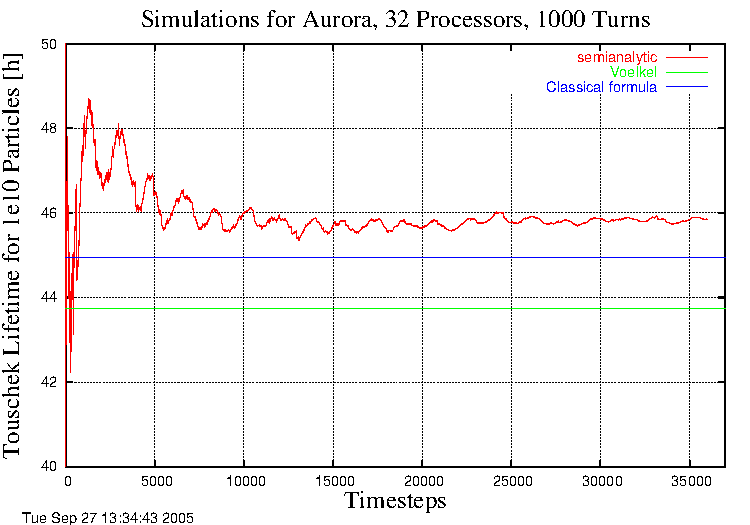
\includegraphics[width=0.80\textwidth]{aurlong.pdf}
 \caption{Aurora Simulation}
\end{figure}
The not falling together with the result from the formulas can be also expected, since these formulas use one fixed beam geometry, and in our simulation the beam geometry is changing.\\
The newer results shows, that for different $\gamma$ the deviation of the V\"olkel and the ZAP calculations are bigger, then the ones from our model.\\
In the following we will compare our different ways of computing the lifetime. Since also these results differ from each other.

\subsection{Semianalytic vs. Analytic}
\begin{figure}[here]
 \centering
 \includegraphics[width=0.80\textwidth]{sls-conv-1.pdf}
 \caption{Longterm Behavior}
\end{figure}
This figure shows that the analytic and semi-analytic approaches of computing the scattering rates stay very close to each other. It also shows that the semianalytic approach has a much better convergence, then the full analytic one. This is probably caused by the particles being picked out at places of statistical importance. It might be worth a try switching from an uniform random number generator to a gaussian one, dropping the densities, and test if we have better convergence with still the same result.\\
For other settings (Aurora simulation), we had full convergence between analytic and semianalytic cases. The non-convergence here might be due to not long enough computation times.
\subsection{2 Particle Approach}
\begin{figure}[here]
 \centering
 \includegraphics[width=0.80\textwidth]{sls-conv-2.pdf}
 \caption{Longterm Behavior}
\end{figure}
The difference between the 2 particle version and the analytic ones, is that the second momenta is taken in the analytic ones where the interaction takes place, for the 2 particle one, we have the probability of finding the momenta somewhere in the beam. This means that it might be interesting to test what happens if we pick particles that are close to each other.

\subsection{Known Drawbacks}
\begin{itemize}
\item We are only simulating Touschek loss, other effects as scattering from residual gas influence the lifetime.
\item If a part of a particle is lost, it is not taken out of the beam.
\item We have no synchrotron radiation.
\item We are only using linear optics.
\end{itemize}

\subsection{Units}
In the simulation the following units are being used. The spatial coordinates are given in meter. The momentum coordinates are given as relative coordinates to a reference momentum. So they are unit less.


\pagebreak
\section{Implementation}
The current implementation of the Touschek Lifetime into a program is called ttrack (Touschek tracker). It is written in C/C++ and is based on $IP^2L$, and is to designed to run fully parallel. You to specify linear lattices and beam geometries in the input file.
\subsection{Scaling}
As the following figure shows the program, doesn't scale very well, as the processor number gets higher. However, this might be due to the particle number being very low. We used $10^5$ particles in the simulation. This means that there are less than 400 particles per processor in average.
\begin{figure}[here]
\centering
 \includegraphics[width=0.80\textwidth]{scaling.pdf}
 \caption{Scaling of ttrack}
\end{figure}

\section{Simulations for SLS}
Using a linear lattice for the SLS, we find for different momenta acceptance the following lifetimes with $6 \cdot 10^9$ particles in the bunch, an RF Voltage of 2.1 kV and an Energy of 2.4 GeV.
\begin{figure}[here]
\centering
\begin{tabular}{l|l}
Momenta Acceptance & Touschek Lifetime \\ \hline
0.5 \% & 0.12 h \\
1.0 \% & 1.01 h \\
1.5 \% & 3.70 h \\
2.0 \% & 8.71 h 
\end{tabular}
\caption{Touschek Lifetime as a function of Momenta Acceptance}
\end{figure}
These computations were done using a matched beam comparable to the current one in the SLS.
\begin{figure}[here]
 \centering
   \includegraphics[width=0.80\textwidth]{sls-acceptance.pdf}
 \caption{SLS Acceptance vs Lifetime}
\end{figure}
\subsection{Simulation vs. Experiment}
As you can see on the figure, the simulated Touschek Lifetimes are longer then the ones in the experiment. This can be due to several effects, as changes in the bunch shape due to non-linear effects, like the quadruples, or shortening from the lifetime caused by scattering at the residual gas.\\
Another reason is that cutting into the momentum acceptance using a scrapper only reduces the momentum acceptance at one place. For the momentum acceptance computed using our program we assume, that it is the same everywhere.
\section{Low Emittance studies}
On the ``Workshop on small emittance lattices'' in March 2004,  Mikael Eriksson speculated that the Touschek Lifetime goes up as the emittance goes down. This is what we are studying here.For the emittance $\epsilon$ of the beam, we have:
\begin{equation} \epsilon \rightarrow \frac \epsilon F \end{equation}
Where F is factor greater then one. We are scaling the bunch geometry, as follows:
\begin{eqnarray}
\sigma_x &\rightarrow& \frac{\sigma_x}{\sqrt F} \\
\sigma_{x'} &\rightarrow& \frac{\sigma_{x'}}{\sqrt F} .
\end{eqnarray}
The justification for this, is that $\sigma_x = \sqrt{\epsilon_x \cdot \beta_x}$, and our $\beta$-function stays constant as we change the emittance.
\begin{figure}[here]
 \centering
   \includegraphics[width=0.80\textwidth]{emi.pdf}
 \caption{Low Emittance Studies for SLS} 
\end{figure}
This figure confirms what Michael Eriksson assumed, the Touschek Lifetime goes up, with ultralowemittance.\\
Values for ultralowemittance show bad convergence behavior, because the event number is low. However, one event counts a lot, because the densities are very high.
\subsection{Comparison with the classical formula}
For the Aurora lattice with its high symmetry, we can run both the classical formula. We have done this, as you can see on the next figure.
\begin{figure}[here]
 \centering
   \includegraphics[width=0.80\textwidth]{emiaur.pdf}
 \caption{Low Emittance Studies for Aurora}
\end{figure}
You can see that, till a factor $F = 10^4$ the classical formula and our simulation predict the same behavior, but then the classical formula goes up much more quickly.

\section{Future Work}
\subsection{Improving the program}
The current model has several drawbacks, but there are possible solutions. Here is a list of some of them.
\subsubsection{Weighting the particles}
At the moment our model only calculates the Touschek Lifetime, but does not calculate how the Touschek Effect affects the beam. To implement this we could give each particle a weight $Q_i$ telling us, how much is left out of the macro particle (we are usually simulating less particles then there are in the real beam.) On each collision we will then reduce the number $Q_i$ by something depending on the cross section of the scattering $\sigma$. So for example:
\begin{equation} Q_i \rightarrow Q_i \cdot f(\sigma) \end{equation}
Here $f(\sigma)$ is a function of the scattering angle (and maybe other things). However one has to take into account that our simulation times are very small compared to the lifetime. The lifetime is in the hours and our simulation times in the microseconds. So probably the effect one will see is very small.
\subsubsection{Include Synchrotron Radiation, Non-linear Optics, residual gas scattering and Polarizations}
Synchrotron Radiation changes the shape of the beam, since the shape of the beam influences the lifetime, including this radiation will change the computed lifetime. The same reasoning applies to non-linear optics and residual gas scattering.\\
Beam Polarization will change the scattering cross section. Since our lifetime depends on this cross section including it will also change our lifetime.
\subsubsection{Use a gaussian random number generator}
As speculated in the section comparing the semianalytic to the analytic computation, using a gaussian random number generator will probably lead to much better convergence.
\subsubsection{Use a 6D Mesh}
At the moment we are using an analytical formula to determine the particle densities in phase space, depending on the Twiss Parameters. However we could also directly determine these densities from our simulation, using a mesh. However, this would mean having a mesh in the phase space, which is 6 dimensional.

\subsection{Investigate the different models}
As described in the simulation part, we have 3 different models to compute the Touschek Lifetime (analytic, semi-analytic and 2 particles). These are giving different results. It might be interesting to investigate why.

\subsection{Changing the model}
It would be nice to model the real motion of the particles, so making the model less Monte Carlo and more deterministic. This is what we first tried to do, but failed. So it is still left for the future.

\subsection{Variable momentum acceptance}
At the moment, we suppose the momentum acceptance is the same around the whole beam line. However this is not the case, so we might need to consider adding a variable momentum acceptance for the beam line, specified in the lattice file.

\section{Acknowledgments}
I would like to thank Andreas Adelmann and Andreas Streun for their great help and support. Additional thanks go to Michael B\"oge and Roman Geus for their help. Without their help, I would certainly not been able to finish this project, and also for allowing me to work with equipment like the Cray-XT3 ``Horizon'' or to be part of doing measurements using the SLS.

\appendix
\begin{thebibliography}{77}	

\bibitem{1} Physics of Nonneutral Plasmas, Ronald C. Davidson, Imperial College Presse, 2001 %1
\bibitem{2} Theory and Design of Charged Particle Beams, Martin Reiser, John Wiley \& Sons, 1994 %2
\bibitem{3} Momentum acceptence and Touschek lifetime, Andreas Streun, SLS Notes 1997 %3
\bibitem{4} Simulation of the Touschek Effect for BESSY II - A Monte Carlo Approach by S. Khan, EPAC 94 %4
\bibitem{5} Basic Course on Acceleratror Optics, J. Rossbach and P. Schmueser %5
\bibitem{6} Coulomb Interactions in Particle Beams, G.H. Jansen % 6
\bibitem{7} Weighted Particles in Coulomb Collision Simulations Based on the Theory of a Cumulative Scattering Angle, K. Nambu and S. Yonemura published in Journal of Computional Physics 145, 639 - 654 (1998) % 7
\bibitem{8} A Binary Collision Model for Plasma Simulation with a Particle Code, Tomonori Takizuka, Journal of Computional Physics 25, 205-219 (1977) %8
\bibitem{9} Particle simulations of plasma, John M. Dawson, Reviews of Modern Physics, Vol. 55, No. 2, April 1983 %9
\bibitem{10} Simulation of the Touschek Effect for Bessy II - a Monte Carlo Approach by S.Khan in Bessy TB Nr. 177/93 %10
\bibitem{11} Particle Loss by Touschek Effect in a s Storage ring, Uta V\"olkel, DESY 67/5 %11
\bibitem{12} ``The top 10 of open questions'', Workshop on small emittance lattices, Lund 10-12 March, 2004, http://maxsun5.maxlab.lu.se/maxlab/conference/small-emittance/presentations/streun/top10.html %12
\bibitem{13} Quantum Electrodynamics, R.P. Feynman, W.A.Bernjamin, Inc, New York 1961 %13
\end{thebibliography}

\end{document}
